% 
% NTHU Template
% 2014 Yao Wei
%
% This file is licensed under CC0.
% https://creativecommons.org/publicdomain/zero/1.0/
%

\documentclass[12pt]{article}

% Lint
\RequirePackage[l2tabu, orthodox]{nag}

% Fonts
\usepackage{mathptmx}
\usepackage[T1]{fontenc}
\usepackage{CJKutf8}

% Layout
\usepackage[a4paper, top=2.54cm, bottom=2.54cm, left=3.17cm, right=2.54cm]{geometry}
\usepackage{abstract}

% Paragraph
\usepackage{indentfirst}
\usepackage{setspace}

\usepackage{tabularx}

% Watermarks
\usepackage{wallpaper}
\CenterWallPaper{.18}{./assets/nthu_watermark.eps}
\setlength{\wpXoffset}{0.315cm}

% Citations

\usepackage[backend=bibtex,sorting=none,maxcitenames=2,maxbibnames=3,hyperref=true,block=none]{biblatex}
\bibliography{thesis}
\renewbibmacro{in:}{}

% Figures
\usepackage{float}
\usepackage{subcaption}
\usepackage{rotating}

% algo
\usepackage{algorithm}
\usepackage{algorithmicx}
\usepackage{amsmath}
\usepackage{algpseudocode}
\algdef{SE}[DOWHILE]{Do}{DoWhile}{\algorithmicdo}[1]{\algorithmicwhile\ #1}%

\renewcommand{\algorithmicrequire}{\textbf{Input:}}
\renewcommand{\algorithmicensure}{\textbf{Output:}}
\newcommand{\var}[1]{\text{\texttt{#1}}}
\newcommand{\func}[1]{\text{\textsl{#1}}}

\makeatletter
\newcounter{phase}[algorithm]
\newlength{\phaserulewidth}
\newcommand{\setphaserulewidth}{\setlength{\phaserulewidth}}
\newcommand{\phase}[1]{%
    \vspace{-1.25ex}
        % Top phase rule
    \Statex\leavevmode\llap{\rule{\dimexpr\labelwidth+\labelsep}{\phaserulewidth}}\rule{\linewidth}{\phaserulewidth}
    \Statex\strut\refstepcounter{phase}\textit{Phase~\thephase~--~#1}% Phase text
            % Bottom phase rule
    \vspace{-1.25ex}\Statex\leavevmode\llap{\rule{\dimexpr\labelwidth+\labelsep}{\phaserulewidth}}\rule{\linewidth}{\phaserulewidth}}
\setphaserulewidth{.7pt}
\makeatother


% math
\usepackage{textcomp}

\begin{document}
\begin{CJK}{UTF8}{bkai}

\begin{titlepage}
\begin{center}
\Huge 國~立~清~華~大~學 \\ [1.5ex]
\Huge \underline{碩~士~論~文} \\
%\Large (初稿)\\
\vspace*{10ex}
\huge DeAr: 適用於異質系統架構之高效率數位訊號處理器資料路徑設計 \\
\vspace*{1ex}
\huge DeAr: An Efficient DSP Datapath Design for Heterogeneous System Architecture  \\

\null
\vfill

\Large
\begin{tabular}{rl}
    \makebox[4em][s]{系\hspace{\fill}所\hspace{\fill}別}:&電機工程學系碩士班\ \ \large{組別:系統組}\\ [1.5ex]
    \makebox[4em][s]{學號姓名}:&103061568~李齊明~(Chi-Ming~Lee)\\ [1.5ex]
    \makebox[4em][s]{指導教授}:&許雅三~博士~(Prof.~Yarsun~Hsu)
\end{tabular}
%\end{tabular}

\vspace*{2ex}
\Large 中華民國 105 年 6 月
\end{center}
\end{titlepage}

\doublespacing
\pagenumbering{roman}
\setcounter{page}{3}
\addcontentsline{toc}{section}{Abstract}

\renewcommand{\abstractnamefont}{\normalfont\bfseries}
\renewcommand{\abstracttextfont}{\normalfont}
\setlength{\absleftindent}{0pt}
\setlength{\absrightindent}{0pt}

\begin{abstract}  % Abstract
	Will be done last.
\end{abstract}
\clearpage
\addcontentsline{toc}{section}{Acknowledgements}

\begin{center}
\textbf{Acknowledgements}
\end{center}
Acknowledgements Page
\clearpage

\singlespacing

\tableofcontents  % Table of contents
\clearpage
\addcontentsline{toc}{section}{List of Figures}
\listoffigures  % List of figures
\clearpage
\addcontentsline{toc}{section}{List of Tables}
\listoftables  % List of tables
\clearpage
\addcontentsline{toc}{section}{List of Algorithms}
\listofalgorithms  % List of tables
\clearpage

\doublespacing
%\setlength{\parskip}{12pt}

\pagenumbering{arabic}

\section{Introduction}

    \subsection{Motivation}
        As wireless communication standard evolves, the demand for a digital signal processing platform that supplies computation with high-performance, high-flexibility and low-energy consumption is gaining momentum in the mobile industry. 
        Take an example of LTE-advance, which is considered to be the next mainstream mobile wireless technology, it provides 10 times higher transmission throughput than that of LTE \cite{lte}. 
        In order to achieve this enhancement, strategies such as scaling up MIMO system and permitting carrier aggregation \cite{carrier} that require more sophisticated arithmetics are adopted in LTE-advance.
        Moreover, these algorithms used in LTE-advance demodulation will still change frequently with the protocol specification.
        Consequently, both energy efficiency and flexibility become crucial considerations in the filed of digital signal processor implementation. 
        However, VLIW and ASIP, which have been popular choices of state-of-the-art digital signal processor (DSP) micro-architecture, serve as two extremes cases for hardware designers who would like to trade-off between flexibility and energy efficiency. 
        VLIW gains good flexibility by allocating each functional unit dedicated control signals and ports on register file that result in significant power dissipation, so it could work orthogonally with each other; 
        On the contrary, ASIP benefits from optimized data-path for the specific ISA or algorithm by sacrificing its flexibility so good energy efficiency is achieved. 
        Consequently, improving energy efficiency while keeping hardware flexibility for DSP on mobile devices becomes a challenge.	
        \\\indent 
        On the other hand, heterogeneous computing, which is referred to systems equipped with multiple types of processors, has opened a new era for digital signal processing. 
        Such an integration of different processors gains performance improvement by taking advantage of particular processing activities to handle certain types of tasks.
        Nowadays, a digital signal processing platform typically contains a CPU that handles control intensive tasks and a DSP that perform computation intensive ones.
        Nevertheless, in such heterogeneous DSP platforms, there is still a drawback owing to the communication latency between processors. 
        Frequent data transfer and task dispatching control between DSP and CPU lead to a  bottleneck of performance. 
        As a result, HSA foundation, found by AMD, ARM, MediaTek, etc, propose a new standard for heterogeneous computing, HSA system specification \cite{systemspec}, to address the problem. 
        The standard creates concepts of unified memory space and architectural queuing language that alleviate burdens on data transfer and task dispatching, becoming the potential mainstream of computer architecture in the future \cite{mainstream}.

    \subsection{Goal and Contribution}
        To improve performance and energy efficiency as well as maintain flexibility for digital signal processing platforms, 
        we present DeAr: A Dual-thread Architecture design for DSP datapath that combines advantages of both VLIW and TTA.
        We also illustrate a framework which integrates DeAr with HSA platforms, which are able to reduce communication overhead between CPU and DSP. 
        Prominent features of DeAr include:
        \begin{itemize}
            \item The VLIW-style datapath enables two threads to execute concurrently. High operations per cycle (OPC) can be achieved with proper compiler scheduling.
            \item TTA-style transport-triggered scheduling aggressively forwards data from accumulators to functional units. Unnecessary data write back (WB) can be avoided so energy dissipation in register file is consequently reduced.
            \item Banked organization of register file eliminates redundant connections from ports to registers. Compared with the conventional centralized organization, both power consumption and circuit area are saved.
            \item Register file access is regularized to a queue/stack operation (i.e. push or pop) instead of conventional random access, which requires more bits to specify a register address. Density of VLIW-style code can be improved.
            \item DeAr is suitable for clustering and it can be scaled up to SIMD or vector-processing architectures to meet the throughput requirement.
        \end{itemize}
        In addition, to evaluate DeAr with existing architectures, we selected several classical DSP kernels \cite{dspstone} \cite{bdti} as the benchmark and use the UMC 65nm CMOS technology to implement the hardware.

        The main contribution of this work is achieve at two levels: micro-architecture and HSA level. 
        On the micro-architecture side, with equal resources of functional unit and register file, DeAr outperformed by 30\% in MOPS\/mW and improve 50\% in code density while remaining competitive computational throughput, compared with the conventional VLIW architecture.
        On the HSA side, we present a completed code generation flow for DeAr which meets the requirements from HSA standard, and illustrate a system framework for exploiting the power of DeAr in an HSA platform.
 
    \subsection{Organization}
        The remainder of this thesis is organized as follows: In Chapter 2, we briefly review work related to our architecture. In Chapter 3, we introduces background knowledge about this work. In Chapter 4, we look into the details of the proposed design. In Chapter 5, we provide experimental results that demonstrate the capabilities of this architecture. Finally, Chapter 6 present conclusions and future work of the thesis.

\newpage

\section{Related Work}
    In the stream of DSP design, many studies have been conducted on register file (RF) organization as it becomes the dominating factor of cycle time, power consumption and chip area \cite{register}.
    Rixner \textit{et al.} indicated that, for conventional centralized organization, the cost grows significantly with the number of functional units (FUs) \cite{register}, posing a serious challenge to VLIW DSP design.
    A straightforward solution to it is partitioning the centralized RF into several parts, each of which serves specific FUs, such as \cite{cluster}.
    Studies like \cite{synzen} and \cite{dsplite} went even further by discarding the centralized RF and allocating each FU a dedicated one, which is also known as distributed RF organization.
    However, dividing RF leads to more complicated compiler design and overhead of inter-RF data transport.
    In addition, above approaches still suffer from poor code density, which is an inherent problem from the VLIW architecture.
    \\\indent
    Some approaches avoided the aforementioned cost growth by customizing the data-path and limiting the number of ports on RF.
    Ou \textit{et al.} proposed composite FUs for DSP, which cascade FUs with a specific order and demand fewer ports on RF \cite{cascade} \cite{hearaid}.
    Similar techniques are often applied to ASIP design but they usually lack flexibility to target general purposes.
    There are further researches that achieve power reduction on RF by minimizing the number of accesses to it.
    Chen \textit{et al.} proposed a simulated-annealing based scheduling that aggressively forwards data from FU outputs to inputs instead of accessing RF \cite{multistage}.
    \cite{move} presented a processor framework: MOVE, which features the separation of data transport and operation in the data-path. 
    The user can program the bypass network in MOVE, and avoid most of accesses to RF by clever data transport.
    Such an architecture that manipulates data transport usually refers to transport-triggered architecture (TTA).
    The Work from Lama \textit{et al.} \cite{ttagpu} also demonstrated a framework that takes the advantage of TTA in graphic processing unit (GPU), and this idea is a potential alternative for DSP design.
    \\\indent
    On the other hand, one may notices that none of the above implementations adopts HSA \cite{systemspec}, which is a promising standard for embedded DSP platforms.
    So far, most of studies on HSA focus on the integration of CPU and GPU. \cite{hsaemu} presented a full system emulator for HSA platforms that include CPUs and GPUs.
    Beyond emulation, \cite{hsacyc} further illustrated a cycle-accurate HSA simulator that integrates QEMU \cite{qemu} and GPGPU-sim \cite{gpgpusim}.
    To the best of our knowledge, little or no research has been performed to apply the standard to DSP platforms.

\newpage

\section{Background}

    \subsection{Evolution of Digital Signal Processors}
        A digital signal processor (DSP) is an optimized computer design that aims at accelerating digital signal processing, such as baseband demodulation or video codec.
        In principle, a programmer extracts routines or algorithms from applications and accelerates them with a DSP.
        Such pieces of code that executed by DSPs are also referred to DSP kernels.
        Unlike general purpose computers, which usually feature powerful ISA and novel branch predictors that help them dealing with control intensive tasks very well,
        DSPs simply focus on computation intensive tasks delivered by another unit (general purpose processor, analog to digital converter, etc.), 
        and thus its hardware can be simplified and optimized for better power efficiency, which enable them to be widely used in mobile devices and embedded systems.
        \\\indent
        The single-issue reduced instruction set computer (RISC), introduced in 1980s \cite{risc}, becomes a popular template for DSP owing to its simplicity.
        The key concept of RISC is designing an ISA with primitive and orthogonal instructions which demand simpler datapath.
        By taking the advantage of the regularity in the datapath, pipelining technique can thus be adopt to achieve the application requirement.
        However, two drawbacks still exist in single-issue RISC. 
        The first is lack of instruction-level parallelism (ILP). 
        Functional units are not able to work concurrently due to the limitation of the single-issue datapath.
        This can be resolved by designing a multi-issue datapath with either hardware (i.e., superscalar) or software scheduling (i.e., VLIW).
        In the field of DSP design, adopting the VLIW architecture is a preferable strategy, 
        because hardware simplicity matters than portability and many optimization approaches can be applied in compilation stages. 
        Figure~\ref{fig:vliw} illustrates a basic VLIW datapah, where multiple instructions can be executed at a cycle.
        The number of ports on RF is scaled up with the issue-width, and the compiler is responsible for performing static scheduling to avoid resources conflict among operations.
        \begin{figure}[!ht] 
            \caption{A basic VLIW datapah}
            \centering
            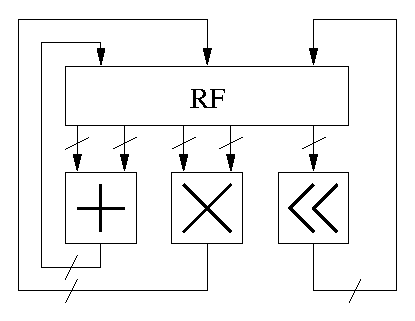
\includegraphics[width=0.5\textwidth]{./figs/vliw.eps}
            \label{fig:vliw}
        \end{figure}
        \\\indent
        The second drawback is plenty of redundant write back (WB). 
        In digital signal processing, intermediate results are often read exactly once, which implies lots of RF storage of them is redundant.
        Several approaches have been proposed to address this issue.
        Figure~\ref{fig:cascade} shows a datapath with a customized composite FU that cascades primitive FUs. 
        Intermediate results can be forwarded from one to its follower with an optimized order which targets specific applications.
        Processor with such customization is referred to application-specific instruction set processor (ASIP).
        \begin{figure}[!ht] 
            \caption{A datapath with a composite functional unit}
            \centering
            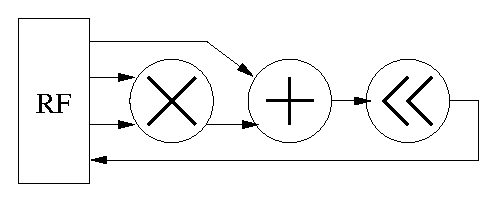
\includegraphics[width=0.6\textwidth]{./figs/cascade.eps}
            \label{fig:cascade}
        \end{figure}
        \\\indent
        Another approach that enables forwarding mechanism even further is shown in Figure~\ref{fig:tta}, where FUs, RF and load/store units are linked by an interconnection network (ICN).
        Such an architecture makes a significant distinction from RISC because only a "move" instruction is needed. 
        All computation can be completed by moving operands on the interconnection network, avoiding WB as much as possible.

        \begin{figure}[!ht] 
            \caption{Transport triggered architecture (TTA)}
            \centering
            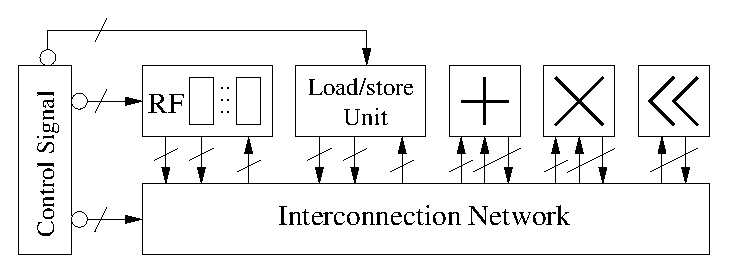
\includegraphics[width=0.8\textwidth]{./figs/tta.eps}
            \label{fig:tta}
        \end{figure}
      
        %\subsubsection{Application-Specific Instruction Set Processor}
        %\subsubsection{Very Long Instruction Word Processor}
        %\subsubsection{Transport-Triggered Architecture}

    \subsection{Register File Model}
    Register file (RF) organization also serves as an important role in DSP design. 
    Increaing computational demand drives more and more FUs on RF,
    which result in significant hardware cost.
    In this part, we will introduce a basic RF model to explain hardware cost in area, delay and power perspectives.
    \subsubsection{Area}
    \label{sec:area}
    RF is an array of register cells, each of which connects to several bit lines and word lines.
    Figure~\ref{fig:rf} illustrates a basic schematic of a register cell.
        \begin{figure}[!ht] 
            \caption{Register cell schematic}
            \centering
            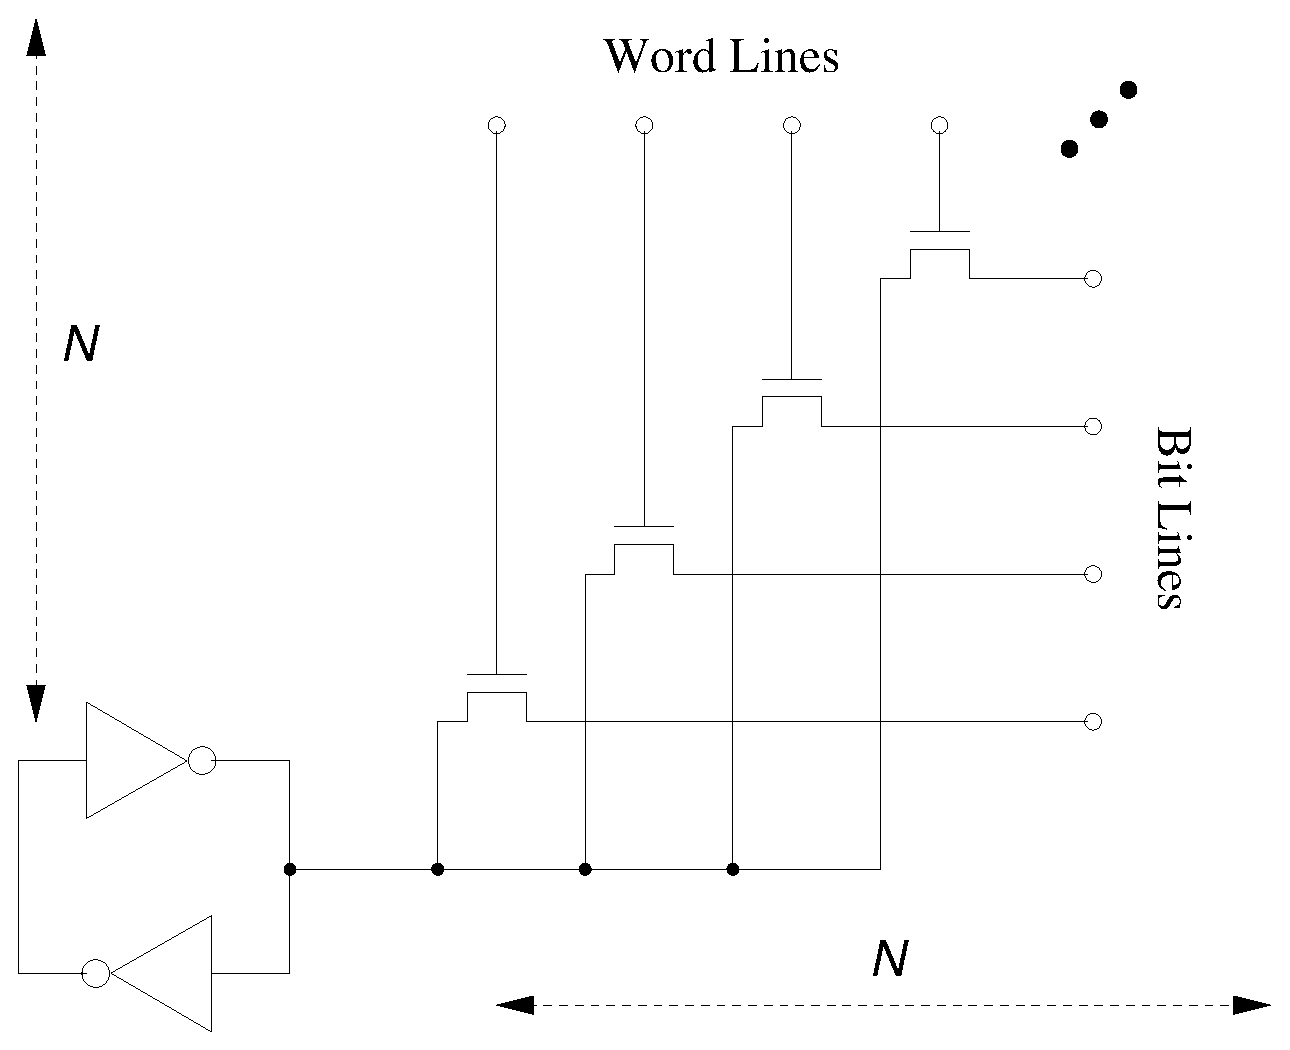
\includegraphics[width=0.7\textwidth]{./figs/rf.eps}
            \label{fig:rf}
        \end{figure}
    For a centralized RF organization with N ports, 
    each register cell is connected to N bit lines, each of which controlled by a word lines.
    N bit lines and N word lines are placed horizontally and vertically respectively.
    Since the width of wire tracks is a constant, 
    the interconnection area of each cell grows with the factor of $N^2$.
    Moreover, since the register number grows with the FU number as well,
    the factor of total interconnection area is further multiplied with another N and reaches $N^3$,  
    which dominates the chip area when N is large.
    \subsubsection{Delay}
    Wire propagation and fan-out/fan-in delays are two major constituents of RF access delay.
    The former is the latency of a logic passage across a wire,
    which is proportional to the wire length, 
    while the latter is the latency of driving on capacitive loads.
    As discussed in ~\ref{sec:area}, the interconnection area of RF is the factor of $N^3$.
    By taking square root on the factor of area, 
    we obtain another factor, $N^{3/2}$, for wire length and propagation delay.
    The growing wire length increases load capacitance on bit lines as well, 
    and it contribute additional fan-out/fan-in delay to the overall.
    Nevertheless, $N^{3/2}$ is still the dominating factor of RF access delay when N is large.
    \subsubsection{Power}
    For each access to RF, bit lines need to be pre-charged to a threshold voltage,
    and then sense register cells by asserting specific word lines.
    As a result, the energy dissipation in RF is mainly resulted from logic switching in bit lines capacitance,
    because every bit line dedicated to a port needs to be active to accomplish an access to the port.
    As the port number increases, the capacitance in bit line is principally wire capacitance.
    The overall power consumption of bit lines grows with the product of the bit line number and the wire length.
    As shown in Figure~\ref{fig:rf}, the wire length and the bit line number of each cell are proportional to N.
    Since the register cell number is proportional to N as well, 
    the overall power consumption of bit lines is also the factor of $N^3$ when N is large.
        %\subsubsection{Centralized Register Files}
        %\subsubsection{Banked Register Files}
        %\subsubsection{Clustered Register Files}
        %\subsubsection{Distributed Register Files}
    \subsection{Heterogeneous System Architecture}
    Heterogeneous System Architecture (HSA) presents an integrated view of various computing devices, 
    such as CPU, DSP, GPU and FPGA.
    HSA allows these devices to be coupled in a single system heterogeneously, and even share the same memory physically.
    Such asymmetry of computing devices in HSA is the key differentiation from conventional symmetric multiprocessing (SMP) \cite{parallel},
    which involves two or more identical processors collaborating with uniform access to the shared memory.
    By adopting HSA, one is able to design a single system that handles wide variety of computational demands efficiently.
    For example, in 2014, AMD released its fourth generation of the Accelerated Processing Unit (APU), \textit{Carrizo APU} \cite{carrizo}, featuring HSA 1.0.
    As illustrated in Figure~\ref{fig:carrizo}, \textit{Carrizo} is the SoC platform with the 4-core CPU and the GPU with 8 compute units (384 shader cores totally).
    Both of them work with the shared virtual memory (SVM) since their MMUs access an identical page table.
    \textit{Carrizo} enables task sharing without data copy between CPUs and GPUs to achieve greater performance.
    By cleverly choosing the suitable computing device for each task, 
    \textit{Carrizo} can operate more efficiently to save power as well.
    Since the proposed DeAr DSP targets HSA platforms, 
    in this part, we will briefly introduce key features of HSA in three perspectives: 
    system specification, programming model and software infrastructure.
        \begin{figure}[!ht] 
            \caption{Carrizo APU with HSA}
            \centering
            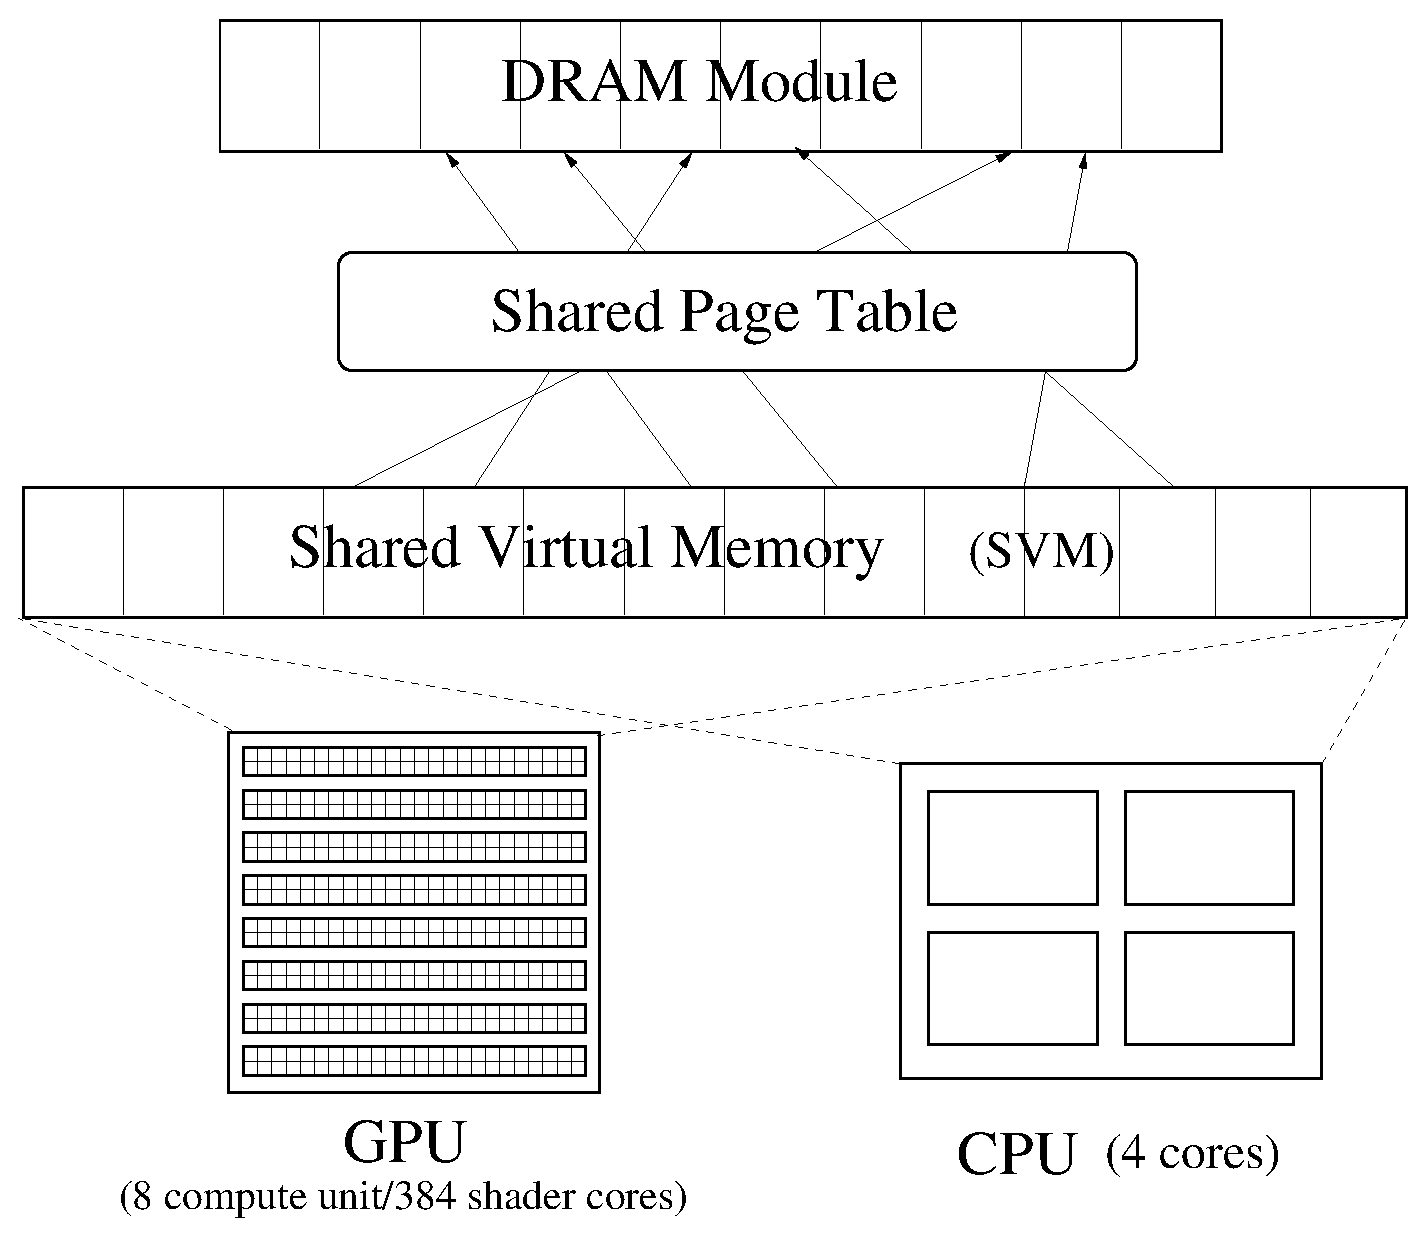
\includegraphics[width=0.8\textwidth]{./figs/carrizo.eps}
            \label{fig:carrizo}
        \end{figure}
        \subsubsection{System Specification}
        The HSA foundation released HSA Platform System Architecture Specification 1.0 \cite{systemspec} in 2015.
        The main purpose of the specification is defining system architecture requirements, 
        which support the HSA programming model and software infrastructure, from a hardware perspective.
        Figure~\ref{fig:systemspec} presents the example of an HSA platform.
        An HSA platform refers to a system involving multiple types of computing devices, 
        which are defined as HSA agents.
        One of the agents needs to be host CPU, and the other usually serve as kernel agents. 
        The host CPU is responsible for running the operating system and setting up \textit{HSA Runtime},
        while kernel agents handle computational tasks from the host CPU by executing HSAIL code.
        HSA require all HSA agents to be capable of accessing SVM maintained coherently, 
        so data exchange between agents can be accomplished by passing data pointer instead.
        Nevertheless, not all memory regions need to be accessible by all agents (i.e., \textit{Global} segment).
        HSA defines other memory segments (\textit{Group}, \textit{Private}, \textit{Spilled}, etc.), 
        which possess various accessibility by various computing agents or items.
        By manipulating different memory segments, the programmer can utilize data locality in memory hierarchy to improve performance.
        To transmit control signals between agents, HSA specifies \textit{Architected Queuing Language} (AQL) as the protocol. 
        AQL defines several packet types: \textit{agent dispatch}, \textit{kernel dispatch}, \textit{AND barrier} and \textit{OR barrier}, etc.
        An agent pushes tasks wrapped in \textit{kernel dispatch} or \textit{agent dispatch} packets to command queues, 
        and other agents consume the packets, and dispatch the wrapped tasks.
        \textit{AND barrier} and \textit{OR barrier} are pushed to command queues to synchronize execution of agents 
        Another advantage of AQL is allowing \textit{user mode queuing},
        which implies the programmer is allowed to access the command queue via \textit{HSA Runtime API} without OS involving.
        By this mean, the latency from dispatching to executing of a task is thus minimized.
        \begin{figure}[!ht] 
            \caption{Example of an HSA Platform}
            \centering
            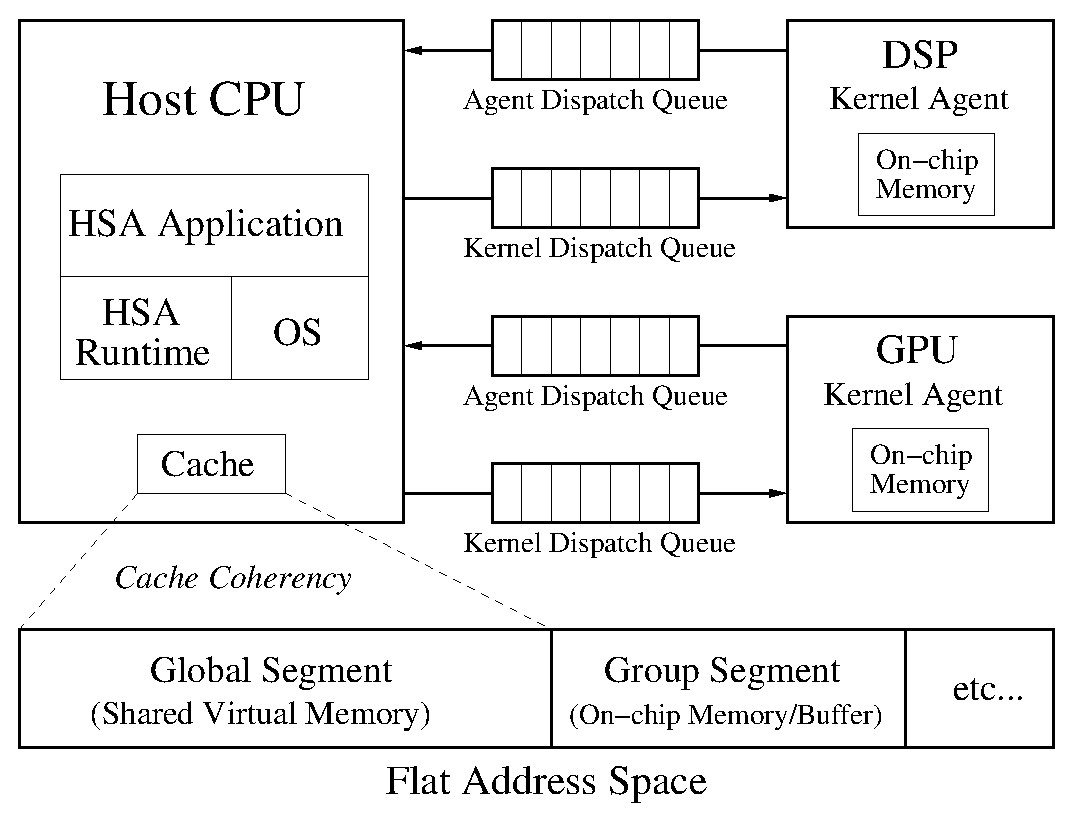
\includegraphics[width=0.75\textwidth]{./figs/systemspec.eps}
            \label{fig:systemspec}
        \end{figure}
        \subsubsection{Programming Model}
        To support multiple Instruction Set Architectures (ISAs) to various agents in a single HSA platform,
        HSA foundation drew up Heterogeneous System Architecture Intermediate Language (HSAIL)
        With HSAIL, programmers can develop code for HSA in an intermediate form accepted by wide range of agents.
        HSAIL basically adopts the parallel programming model of Single Instruction Multiple Data (SIMD), 
        which carries out same computation on different data to accelerate applications.
        HSAIL organizes instances of execution in specified hierarchy, which help programmers to manipulate the SIMD model.
        Figure~\ref{fig:grid} presents a graphical view on how HSAIL organizes instances of execution.
        The atomic instance of execution is work-items, each of which has dedicated registers and private memory.
        Group of work-items form a work-group, which owns group memory accessed by subordinate work-items only.
        The work-items in a work-group can be arranged in one, two or three dimensional coordinate, 
        and the programmer specifies the number of dimensions as well as the size of each dimension.
        Based on the same principle of arranging instances, all work-groups further form a grid, 
        which provides a global view to all work-items created in an HSAIL program (kernel).
        Work-items within a work-group are executed concurrently in chunks called wavefronts, 
        of which sizes are limited by the number of processing cores (lanes) in the target kernel agent.
        Each work-group and each work-item have work-group ID and work-item ID respectively.
        By manipulating such threading hierarchy, 
        the programmer can control accessibility of data and synchronize the work items in a specific scope without burden.
        \begin{figure}[!ht] 
            \caption{Execution hierarchy in HSAIL}
            \centering
            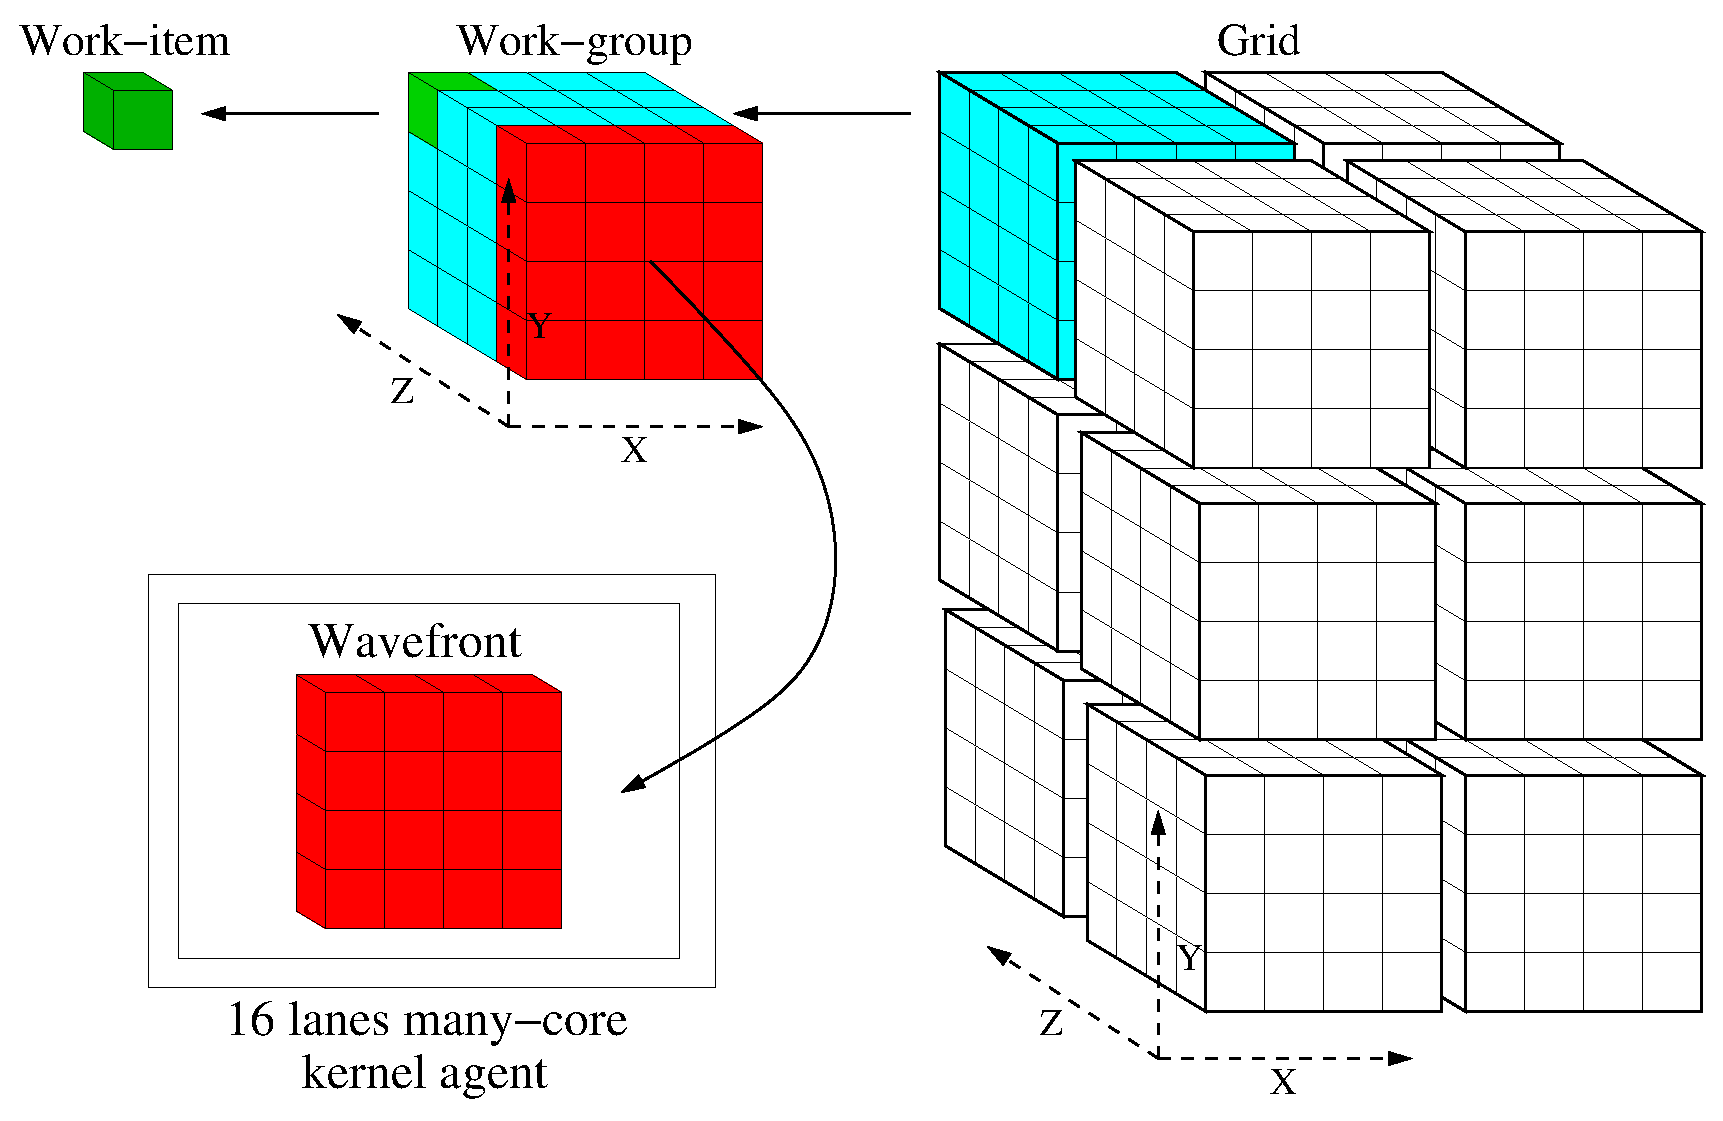
\includegraphics[width=0.85\textwidth]{./figs/grid.eps}
            \label{fig:grid}
        \end{figure}
        % work group, work item warp, memory hierarchy, hqueue, 
        \subsubsection{Software Infrastructure}
        The software infrastructure of HSA is composed of two parts, the compilation tools and the \textit{HSA runtime}.   
        The compilation tools are responsible for generating machine code of specific ISAs from high-level language.
        Figure~\ref{fig:swinf}~(a) illustrates the whole compilation flow of HSA software.
        The programmer develops applications targeting HSA with high-level parallel programming language such as OpenCL, OpenMP or a domain-specific language (DSL).
        The off-line compiler of the hight-level language translate the code to standard HSAIL kernel accepted by all computing devices in an HSA platform.
        Each kind of the computing devices must be recognized by the finalizer, 
        which is composed of several device-specific HSAIL compilers.
        Depending on which device is going to execute the kernel, 
        the finalizer translates the HSAIL to corresponding ISA and completes the code generation flow.
        \\\indent
        On the other hand, the \textit{HSA runtime} bridges HSAIL runtime APIs and agents, as illustrated in Figure~\ref{fig:swinf}~(b).
        With the \textit{HSA runtime}, the programmer is allowed to manipulate system memory and AQL, 
        and thus SVM and \textit{user mode queuing} can be accomplished.
        It is possible that the programmer triggers the finalizer to perform the final stage of compilation at runtime.
        In addition, \textit{HSA runtime} also perform error handling and retrieve system and agent information for users.
        \begin{figure}[!ht] 
            \caption{Software Infrastructe of HSA}
            \centering
            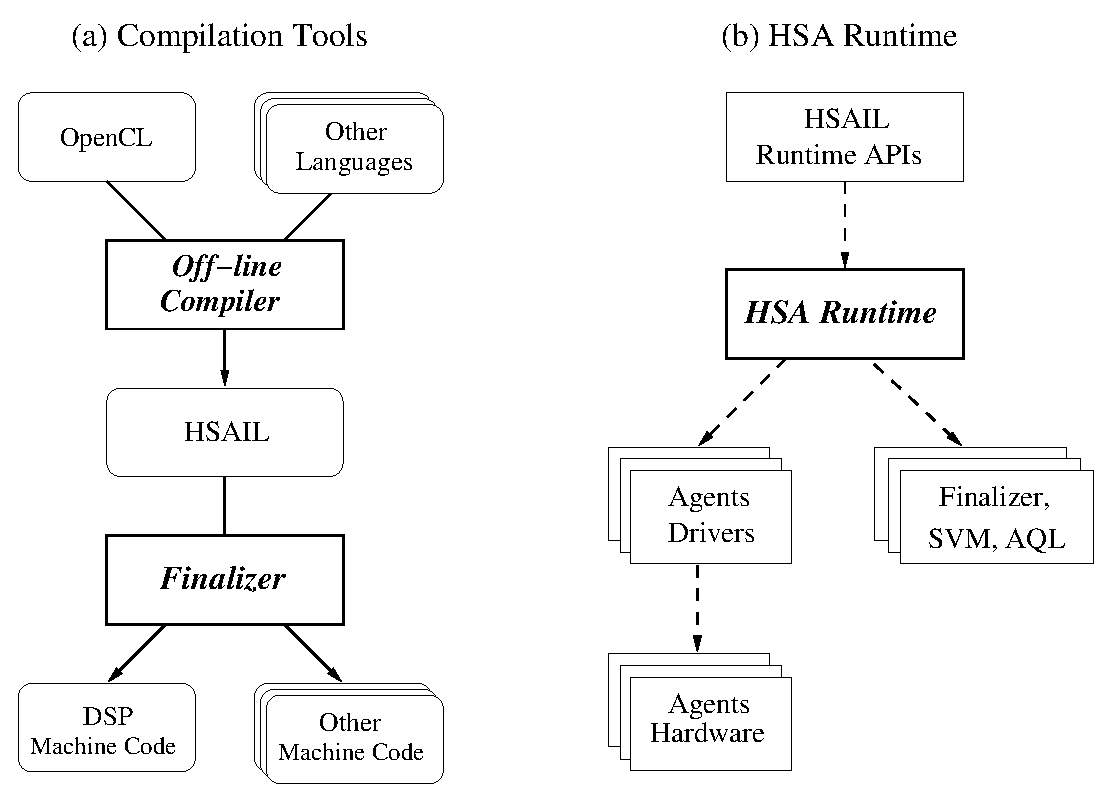
\includegraphics[width=0.85\textwidth]{./figs/swinf.eps}
            \label{fig:swinf}
        \end{figure}
\section{Design and Implementation}
    \subsection{System Overview}
    \subsection{Micro-architecture Design}
        Figure~\ref{fig:micro} demonstrates the micro-architecture of DeAr datapath.
        \begin{figure}[!ht] 
            \caption{Micro-architecture of DeAr}
            \centering
            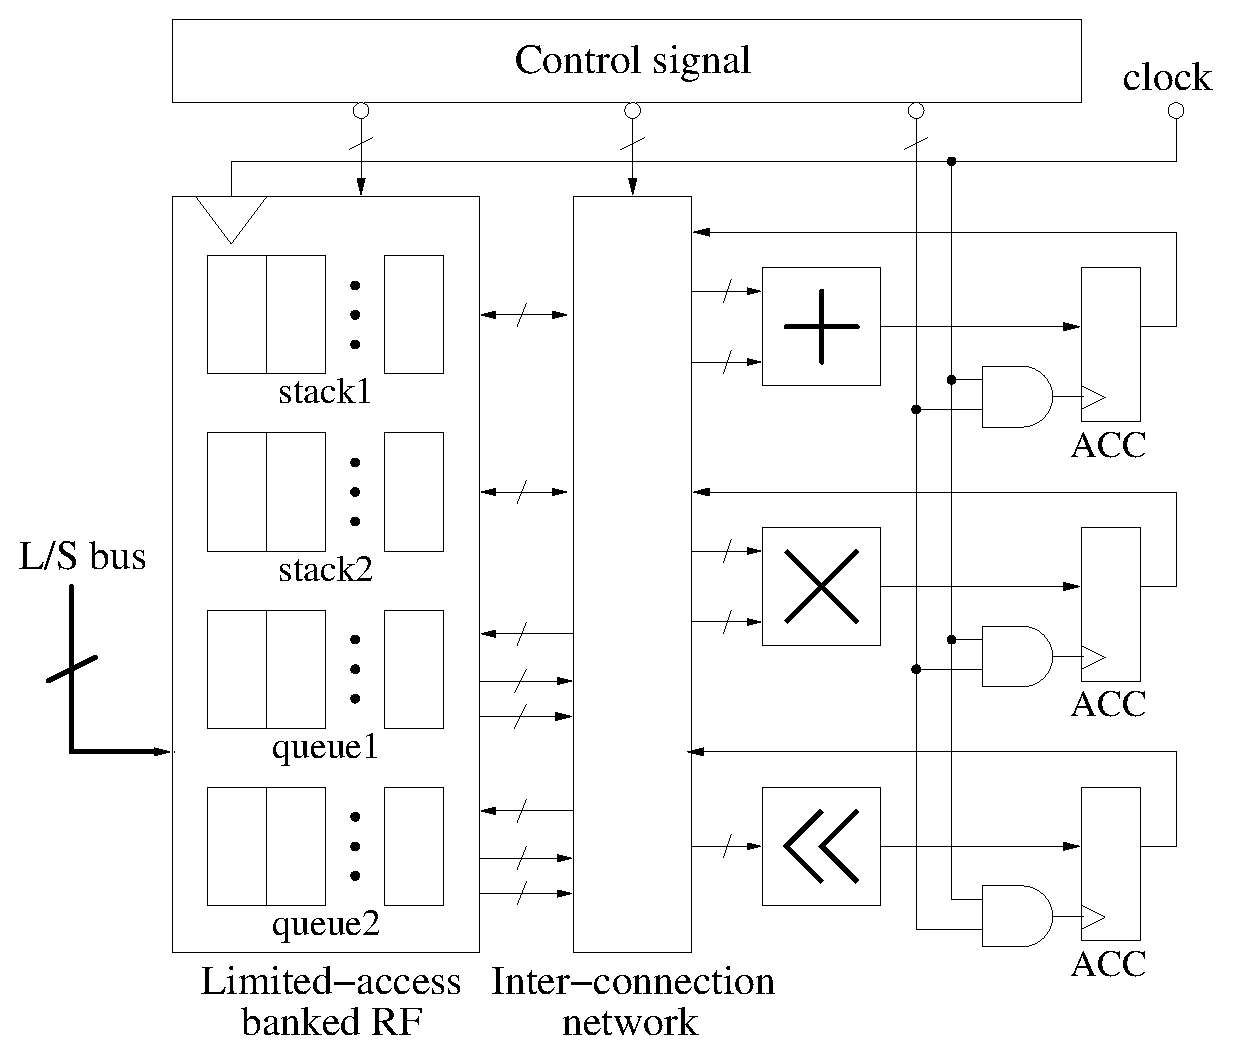
\includegraphics[width=0.8\textwidth]{./figs/micro.eps}
            \label{fig:micro}
        \end{figure}
    \subsection{Software Design}
        \subsubsection{Software framework for DeAr}
            To fully exploit the power of DeAr, we also present a completed code generation flow including compilation, scheduling and optimization.
            Algorithm~\ref{alg:framework} provides an overview of the software framework for DeAr. 
            The user only need to provide DSP kernel code written in OpenCL and a flag which determines the optimization level as the input.
            With CLOC \cite{cloc} tool provided by \textit{HSA Foundation}, the kernel code is converted to standardized HSAIL, $H$, as shown in Line~\ref{line:tohsail}.
            Next, in Line~\ref{line:trans}-\ref{line:trane}, 
            we run the HSAIL transformation (elaborated in \ref{sec:trans}) on HSAIL code and obtain a hierarchical data flow graph (HDFG), 
            $\bar{G}$ (elaborated in \ref{sec:hdfg}), which holds crucial scheduling heuristics.
            After that, in Line~\ref{line:optstart} to \ref{line:optend}, we perform the key part of DeAr software, 
            operation scheduling and optimization (elaborated in \ref{sec:sando}).
            The optimization flag $\lambda$ in Line~\ref{line:forlambda} determines the number of iterations to be used.
            For each iteration, the scheduler exhausts heuristics in $\bar{G}$ which optimize the cycle and WB counts, 
            and it schedules operations with a limited randomness.
            Finally, the scheduler select the scheduling result with the least cycle count, 
            $C_{golden}$ among iterations and generates the final code $X_{golden}$ for DeAr as the output.
            %-----------------framework algo -------------
            \begin{algorithm}[h]
              \caption{\textproc{Software Framework for DeAr}}
              \begin{algorithmic}[1]
                    \Require 
                        High-level DSP kernel code in OpenCL, Optimization flag $\lambda$
                    \Ensure 
                        Binary code of DeAr

                  %\State Convert the kernel code to HSAIL code
                  \State $hsail \Leftarrow$ \Call{CL Offline Compiler }{ $kernel$ }
                  \label{line:tohsail}
                  %\State Perform SSA transformation on HSAIL;
                  %\label{tossa}
                  %\State Convert SSA code to DFG, $G = ( V_{op} , E_{op} )$, where $V_{op}$ is the set of operations and $E_{op}$ is the set of their dependencies;
                  %\label{todfg}
                  %\State Perform hierarchization on $G$, and get $\bar{G} = ( V_{bt} , E_{bt} )$, where $V_{bt}$ is a set of binary trees and $E_{bt}$ is the set of their dependencies;
                  \State $G \Leftarrow$ \Call{Convert HSAIL to DFG by SSA }{ $hsail$ }
                  \label{line:trans}
                  \State $\bar{G} \Leftarrow$ \Call{Hierarchize DFG to HDFG }{ $G$ }
                  %\State Perform the HSAIL transformation on HSIL code, and obtain a HDFG, $\bar{G}$
                  \label{line:trane}
                  \State $C_{golden} \Leftarrow  \infty$
                  \label{line:optstart}
                  \For {$i=1$ to $f(\lambda)$}
                    \label{line:forlambda}
                    %\State Schedule operations in $\bar{G}$ and get binary code $X_i$ and its total cycle count $C_i$
                    \State $X_{inter}, bt_{remain} \Leftarrow$ \Call{Inter-tree Scheduling }{ $\bar{G}$ }
                    \State $X_i, C_i \Leftarrow$ \Call{Intra-tree Scheduling }{ $X_{inter}, bt_{remain}$ }
                    \If {$C_i < C_{golden}$}
                      \State $C_{golden} \Leftarrow C_i$
                      \State $X_{golden} \Leftarrow X_i$
                    \EndIf
                  \EndFor
                  \State Return $X_{golden}$
                  \label{line:optend}
              \end{algorithmic}
              \label{alg:framework}
            \end{algorithm}
            %-----------------------------------------

        \subsubsection{Data Flow Graph and Hierarchical Data Flow Graph}
        \label{sec:hdfg}
            A data flow grahp (DFG), which presents dependencies among operations, is crutial information for program analysis.
            By partitioning a program into basic blocks, the control flow can be simplified, and thus each DFG of a basic block is a directed acyclic graph (DAG).
            Figure~\ref{fig:dfg} illustrates an example of a DFG, where each node and each edge denote an operation and a dependency respectively.
            We can further express any DFG as a data structure $G$, which holds a set of nodes (operations), $V_{op}$, and a set of edges (dependencies), $E_{op}$
            In conventional DSP software design, optimal scheduling of operations is often approached by analyzing DFGs.
            For example, \cite{dsplite} solves ILP problems \cite{ilp} in DFGs in scheduling, 
            and list scheduling \cite{list} calculates scheduling range of operations in DFGs as the scheduling criteria. \\\indent

            However, we found that conventional DFG analysis is infeasible for scheduling in DeAr due to uniqueness of its datapath.
            As a result, in this work, we propose an enhanced version of DFG, hierarchical data flow graph (HDFG), to fit DeAr.

            Figure~\ref{fig:hdfg} demonstrate a HDFG, $\bar{G} = {V_{bt}, E_{bt}}$, converted from Figure~\ref{fig:dfg}.
            We organize several important features of HDFG as below: 
            \begin{itemize}
                \item Cascaded operations, which implies no fork and join of edges within the cascade, are grouped into a super node ($sn$). 
                      If an operation is isolated, it forms a $sn$ directly.
                \item Neighboring $sn$ are further grouped into binary trees, $bt$s, which form a set of vertices, $V_{bt}$, in HDFG.
                      If a $sn$ is isolated, it forms a binary tree directly.
                \item Dependencies among operations that cross binary trees are inherited by binary trees they belong to.
                      These inherited dependencies form a set of edges, $E_{bt}$, among $V_{bt}$.
                \item A $bt$ without any in-edge existing in $V_{bt}$ (i.e., $\sum_{v \in V_{bt}}\textrm{deg}^-(bt) = 0$) is free to be scheduled. 
                      After scheduled, the $bt$ and its edge will be erased from $\bar{G}$.
                \item Every $sn$ must have either zero (leaf nodes) or two (non-leaf nodes) children.
                      Edges in a HDFG at $bt$, $sn$ and operation level guarantee the correctness of execution order.
            \end{itemize}

            The hierarchy of HDFGs can provide crutial optimization heuristics to the DeAr scheduler.
            DeAr avoids RF access within a super node, and regularize RF access into first-in last-out fashion (stack) with the help from the recursive property of a binary tree.
            In addition, the binary property also provides a chance to balance workload for two threads.



        
        \subsubsection{HSAIL Transformation}
        \label{sec:trans}
        The whole process of the HSAIL transformation contains two phases elaborated as below:
        \begin{itemize}
            \item \textbf{Phase 1: Convert HSAIL to DFG by SSA} \\\indent
                Algorithm~\ref{alg:2dfg} illustrates how this phase works.
                Single static assignment (SSA) \cite{ssa} is another form of IR which simplifies work of compiler significantly, 
                and thus deriving the SSA form of the code becomes the first step.
                SSA form specifies that each variable must be assigned exactly once, which is the key distinction from HSAIL.
                \\\indent
                The conversion from normal HSAIL to SSA form is initialized by performing reaching definition analysis \cite{rda} as shown in Line~\ref{line:rda}.
                Next, for each assignment in the code, we give a new name to the LHS variable, and update corresponding new names of RHS variables indicated by reaching definition analysis.
                These iterations which derive the SSA form correspond to Line~\ref{line:forhsails}-\ref{line:forhsaile}.
                Now, each assignment to some variable $X$ denotes an operation, which dominates operations with $X$ appearing in their RHS variables.
                As a result, we can construct the DFG without burden by iterating the new code, as shown in Line~\ref{line:forssas}-\ref{line:forssae}.
                Operations and their dependencies are stored in a set of vertices $V_{op}$ and a set of edges $E_{op}$ respectively, 
                and thus the DFG, $G = ( V_{op} , E_{op} )$, is constructed.
        %----------hsail to dfg algo--------------
        \begin{algorithm}[h!]    \caption{\textproc{Convert HSAIL to DFG by SSA}}
        \begin{algorithmic}[1]
            \Require    HSAIL code
            \Ensure     $G = ( V_{op} , E_{op} )$   \Comment{ DFG }
            \State      Peform reaching definition analysis     \label{line:rda}
            \For        {each assignment (operation) in the HSAIL code}     \label{line:forhsails}
                \State      Give a new name to the LHS variable
                \State      Update RHS variables with corresponding new names in other assignments
                \EndFor                                                     \label{line:forhsaile}
            \State      Initialize $G \textrm{, where } V_{op} = \emptyset \textrm{ and } E_{op} = \emptyset $
            \For        {each assignment (operation) in the new HSAIL code} \label{line:forssas}    \Comment{SSA form}
                \State      Insert the LHS variable $x$ to $V_{op}$
                \For        {each variable $y$ in the RHS}
                    \State      Insert a new edge ($x$, $y$)
                \EndFor
            \EndFor                                                         \label{line:forssae}
        \end{algorithmic}
        \label{alg:2dfg}
        \end{algorithm}
        %----------------------------------------

            \item \textbf{Phase 2: Hierarchize DFG to HDFG} \\\indent
                As discussed in~\ref{sec:hdfg}, an HDFG is an enhanced version of a DFG which provides necessary heuristics for DeAr scheduler.
                Hierarchizing a DFG to an HDFG can be achieved by traversing the DFG, details of which are shown in Algorithm~\ref{alg:tohdfg}.
                In Line~\ref{line:forroots}-\ref{line:forroote}, the algorithm firstly iterates all root operations (i.e., $\textrm{deg}^+(op)=0$ ) in $G$,
                and call the first subroutine, \textproc{Build Binary Tree }, on each root operations.
                Line~\ref{line:bbts}-\ref{line:bbte} show the details of \textproc{Build Binary Tree }.
                A binary tree $bt$ is initialized by building a super node $sn$ on the input operation $op$ with the second subroutine, \textproc{Build Super Node }, 
                which groups cascaded operations ending with $op$, as shown in Line~\ref{line:bsns}-\ref{line:bsne}.
                After that, the third subroutine \textproc{Grow Binary Tree }, described in Line~\ref{line:gbts}-\ref{line:gbte}, will expand $bt$ by including neighboring operations if each of operations has exactly one out-edge (i.e., $\textrm{deg}^+(op)=1$), as shown in Line~\ref{line:growifs}-\ref{line:growife}. 
                \\\indent
                On the contrary, if the aforementioned condition is not met with any of $op_{left}, op_{right}$, 
                it will call \textproc{Build Binary Tree } on both to build new binary trees, $bt_{left}, bt_{right}$,
                and record the new dependencies, $bt_{left} \rightarrow bt, bt_{right} \rightarrow bt$.
                This step is demonstrated in Line~\ref{line:growelses}-\ref{line:growelsee}. 
                \\\indent
                The recursion proceeds by cross-calling between \textproc{Build Binary Tree } and \textproc{Grow Binary Tree } until the whole DFG is traversed.
                Binary trees and their dependencies are stored in a set vertices $V_{bt}$ and a set of edges $E_{bt}$ respectively.
                Finally, the HDFG, $\bar{G} = ( V_{bt} , E_{bt} )$, is constructed and returned.
        \end{itemize}

        %----------DFG to HDFG algo--------------
        \begin{algorithm}[h!]    \caption{\textproc{Hierarchize DFG to HDFG}}
        \begin{algorithmic}[1]
            \Require    $G = ( V_{op} , E_{op} )$ \Comment{ DFG }
            \Ensure     $\bar{G} = ( V_{bt} , E_{bt} )$ \Comment{ HDFG }
            \State      Initialize $\bar{G} \textrm{, where } V_{bt} = \emptyset \textrm{ and } E_{bt} = \emptyset $
            \For        {each of $  op \ni \sum_{op \in V_{op}}\textrm{deg}^+(op) = 0 $}  \label{line:forroots}   \Comment{For each root vertex}
                \State      $v_{bt} \Leftarrow $\Call{Build Binary Tree }{$op$}
                \State      Insert $v_{bt}$ to $V_{bt}$
            \EndFor                                                                    \label{line:forroote}
            \Statex %---------------------------
            \Function   {Build Binary Tree }{$op$}         \label{line:bbts}
                \State      Initialize a birary tree $bt$
                \State      $sn \Leftarrow$ \Call{Build Super Node }{$op$}
                \State      Set $sn$ as the root of $bt$
                \State      \Call{Grow Binary Tree }{$sn$}
                \State      \Return {$bt$}
            \EndFunction                                \label{line:bbte}
            \Statex %--------------------------
            \Function   {Grow Binary Tree }{$sn$}          \label{line:gbts}
                \If         { $\textrm{deg}^-(sn.tail) = 2$ }     \Comment{A branch in the DFG}
                    \State      $op_{left}, op_{right} \Leftarrow op \ni (op \rightarrow sn.tail) \in E_{op}$ 
                    \If         {$\textrm{deg}^+(op_{left}) = \textrm{deg}^+(op_{right}) =1$}  \label{line:deg}  \label{line:growifs}
                        \State      $sn.left\_child \Leftarrow$ \Call{Build Super Node }{$op_{left}$}
                        \State      \Call{Grow Binary Tree }{$sn_{left}$}
                        \State      $sn.left\_child \Leftarrow$ \Call{Build Super Node }{$op_{right}$}
                        \State      \Call{Grow Binary Tree }{$sn_{right}$}     \label{line:growife}
                    \Else       \label{line:growelses}
                        \State      $bt_{new} \Leftarrow$ \Call{Build Binary Tree }{$op_{left}$}
                        \State      Insert the new tree $bt_{new}$ to $V_{bt}$
                        \State      Insert the new edge $(bt_{new} \rightarrow v_{bt})$ to $bt$
                        \State      $bt_{new} \Leftarrow$ \Call{Build Binary Tree }{$op_{right}$}
                        \State      Insert the new tree $bt_{new}$ to $V_{bt}$
                        \State      Insert the new edge $(bt_{new} \rightarrow v_{bt})$ to $bt$ \label{line:growelsee}
                        \EndIf                          \label{line:gbte}
                \EndIf
            \EndFunction
            \Statex %-----------------------
            \Function   {Build Super Node }{$op$}  \label{line:bsns}
                \State  Initialize a super node $sn$ 
                \State  $sn.head \Leftarrow op$
                \While{$\textrm{deg}^-(op) = 1$}
                    \State   $op \Leftarrow op_{next} \ni (op_{next} \rightarrow op) \in E_{op}$ 
                \EndWhile
                \State  $sn.tail \Leftarrow op$
                \State      \Return {$sn$}
            \EndFunction                        \label{line:bsne}
        \end{algorithmic}
        \label{alg:tohdfg}
        \end{algorithm}
        %--------------------------------------

    
        \subsubsection{Scheduling}

        A scheduler is responsible for ensuring the order of operations, 
        arranging data movement and allocating hardware resources.
        Once the scheduling result is determined, the corresponding machine code is also generated.
        The principle of the DeAr scheduler is, 
        two threads process binary trees in a HDFG concurrently and collaboratively until all operations are scheduled.
        Before exploring how threads co-work, we need to look into how a binary tree, $bt$, is handled by the scheduler.
        Algorithm~\ref{alg:sbt}, \textproc{Schedule Binary Tree}, 
        demonstrates how operaions of a $bt$ are scheduled into a specific sequence.
        %-------Schedule Binary Tree----------
\begin{algorithm}[h]
    \caption{\textproc{Schedule Binary Tree }}
    \begin{algorithmic}[1]
        \Require    $sn$
        \Ensure     $list_{op}$
        \If{$sn$ is NOT a leaf node}        \label{line:sbts}
            \State $size_{left} \Leftarrow$ \Call{Stack Size }{$sn.left\_child$}
            \State $size_{right} \Leftarrow$ \Call{Stack Size }{$sn.right\_child$}
            \If{$size_{left} > size_{right}$}
                \State \Call{Schedule Binary Tree }{$sn.left\_child$}
            \Else
                \State \Call{Schedule Binary Tree }{$sn.right\_child$}
            \EndIf
        \EndIf
        \State \Call{Schedule Super Node }{$sn$}   
        \State Erase $sn$ from the binary tree
        \If{$sn$ IS a root node}        
            \State \Return{$list_{op}$}
        \EndIf

        \label{line:sbte}
        \Statex
    \Function   {Stack Size }{$sn$}  \label{line:gsss}
        \If{$sn$ is a leaf node}
            \State $size \Leftarrow 0$
        \Else
            \State $size \Leftarrow \text{\textproc{Max}(\ \textproc{Stack Size }($sn.left\_child$), \textproc{Stack Size }($sn.right\_child$)\ )} + 1$
        \EndIf
        \State \Return{$size$}
    \EndFunction                    \label{line:gsse}
    \Statex
    \Function   {Schedule Super Node }{$sn$}  \label{line:ssns}
       \State   $op \Leftarrow$ $sn.tail$
       \Do   
           \State Insert $op$ to $list_{op}$
           \State $op \Leftarrow op_{next}$
       \DoWhile{$op \neq sn.head$}
    \EndFunction                            \label{line:ssne}

    \end{algorithmic}
    \label{alg:sbt}
\end{algorithm}
    %----------------------------------------------
        It traverse a $bt$ recursively in a post-order fashion, which implies the root is touched first but scheduled last.
        The input is the root $sn$ of a $bt$, and then a list of operations, which indicates execution flow, is returned.
        Line~\ref{line:sbts}-\ref{line:sbte} is the main part of the algorithm.
        For a input $sn$, the existence of its children is checked at the beginning.
        If children exist, the same algorithm, \textproc{Schedule Binary Tree }, is applied to them and the recursion starts.
        The first subroutine, \textproc{Stack Size } shown in Line~\ref{line:gsss}-\ref{line:gsse}, determines the precedence of children.
        After the recursion, the second subroutine, 
        \textproc{Schedule Super Node} shown in Line~\ref{line:ssns}-\ref{line:ssne}, is applied to this $sn$, 
        By this subroutine, cascaded operations in the $sn$ are scheduled consecutively.
        \\\indent
        The key insight of Algorithm~\ref{alg:sbt} is, it optimizes RF access significantly with heuristics from HDFGs.
        Firstly, operations in a $sn$ are scheduled consecutively.
        With this policy, the forwarding mechanism in DeAr can be taken advantage, and unnecessary WB is can be avoided.
        Secondly, the scheduler always schedules the child which demands larger stack size earlier, 
        By this mean, the stack size used by a parent $sn$ is the smaller one of two children plus one, 
        so that we can ensure the cost on stack size is minimized and prevent RF from spilling.
        \\\indent
        We further introduce \textproc{Inter-tree scheduling} and \textproc{Intra-tree scheduling}, 
        both of which require Algorithm~\ref{alg:sbt}.
        A typical HDFG contains multiple $bt$.
        As a result, the DeAr scheduler perform \textproc{Inter-tree scheduling} if multiple $bt$ exist.
        Algorithm~\ref{alg:inter} illustrate the detail of \textproc{Inter-tree scheduling}, 
        where a HDFG, $\bar{G}$ is input, and binary code segment, 
        $X_{inter}$, accompanied with a remaining subtree, $bt_{remain}$, will be returned.
        %-----------Inter-tree-------------
\begin{algorithm}[h!]
    \caption{\textproc{Inter-tree Scheduling}}
    \begin{algorithmic}[1]
        \Require    HDFG $\bar{G} = (V_{bt}, E_{bt})$
        \Ensure     Remaining subtree $bt_{remain}$, binary code segment $X_{inter}$
        \State $X_{inter} \Leftarrow NULL$       \Comment{Initialize $X_{inter}$}
        \While{$V_{bt} \neq \emptyset$} \label{line:interws}
            \If{$work\_queue_{thread1} = \emptyset$}
                \State Select a binary tree $bt \ni \sum_{bt \in V_{bt}}\textrm{deg}^-(bt) = 0$ randomly
                \State $list_{op} \Leftarrow$ \Call{Schedule Binary Tree }{$bt.root$}
                \State Push $list_{op}$ into $work\_queue_{thread1}$
                \State Erase $bt$ and its edges from $\bar{G}$
            \EndIf
            \If{$work\_queue_{thread2} = \emptyset$}
                \State Select a binary tree $bt \ni \sum_{bt \in V_{bt}}\textrm{deg}^-(bt) = 0$ randomly
                \State $list_{op} \Leftarrow$ \Call{Schedule Binary Tree }{$bt.root$}
                \State Push $list_{op}$ into $work\_queue_{thread2}$
                \State Erase $bt$ and its edges from $\bar{G}$
            \EndIf
            \State $X_{inter} \Leftarrow X_{inter} \oplus$ \Call{Gen Code by DP}{$work\_queue_{thread1}$, $work\_queue_{thread2}$} \label{line:intercon}
        \EndWhile \label{line:interwe}
        \If{$work\_queue_{thread1} \neq \emptyset$} \label{line:interis}
            \State $bt_{remain} \Leftarrow$ \Call{Restore Subtree from Queue }{$work\_queue_{thread1}$}
            \State Clear $work\_queue_{thread1}$
        \ElsIf{$work\_queue_{thread2} \neq \emptyset$}
            \State $bt_{remain} \Leftarrow$ \Call{Restore Subtree from Queue }{$work\_queue_{thread2}$}
            \State Clear $work\_queue_{thread2}$
        \Else
            \State $bt_{remain} \Leftarrow NULL$
        \EndIf \label{line:interie}
        \State \Return{$X_{inter}$, $bt_{remain}$}
    \end{algorithmic}
    \label{alg:inter}
\end{algorithm}
        %------------------------------------------
        Line~\ref{line:interws}-\ref{line:interwe} enclosed by a while loop, is the main part of \textproc{Inter-tree scheduling}.
        The scheduler performs several identical steps for thread~1 and thread~2 respectively.
        It firstly search the whole $\bar{G}$ and select a free $bt$ randomly.
        Such a selection preserves randomness for DeAr scheduler, 
        and a better scheduling result is possible to be achieved with more trials, as discussed in Algorithm~\ref{alg:framework}.
        Next, the scheduler checks whether the work-queue of a thread is empty.
        If it is empty, the scheduler processes the selected $bt$ with Algorithm~\ref{alg:sbt}, 
        and enqueue the returned $op_{list}$ to the work-queue of a thread.
        Here, a work-queue is data structure that holds the operation sequence that belongs to a thread.
        An operation is removed from a thread's work-queue once it is indeed dispatched to binary code.
        After above steps, two work-queue are filled, and the key of this algorithm, \textproc{Gen Code by DP}, is performed.
        This subroutine, \textproc{Gen Code by DP}, dispatches operations in two work-queues which execute concurrently to binary code, 
        and arbitrates for FU conflict by Dynamic Programming (DP) \cite{dp}.
        It then returns a new code segment concatenated by the current one, and ensures at least one work-queue is cleared.
        Here, as shown in Line~\ref{line:intercon}, we use the sigh, $\oplus$, to denote the operation of code concatenation.
        Repeat of the loop proceeds until all $bt$ in $\bar{G}$ are consumed.
        However, it is very likely that there is a work-queue where operations remaining at the last iteration.
        Line~\ref{line:interis}-\ref{line:interie} illustrate such a scenario.
        Since the resulting binary code is incomplete, 
        remaining operations are reverted to the part of their original binary tree by \textproc{Restore Subtree from Queue},
        and a remaining subtree, $bt_{remain}$, is returned.
        \\\indent 
        To deal with $bt_{remain}$ and obtain the remaining part of the binary code, 
        \textproc{Intra-tree Scheduling}, illustrated in Algorithm~\ref{alg:intra}, is applied.
        %----------------Intra-tree---------------
\begin{algorithm}[h]
    \caption{\textproc{Intra-tree Scheduling}}
    \begin{algorithmic}[1]
        \Require    Remaining subtree $bt_{remain}$, binary code segment $X_{inter}$
        \Ensure     Final binary code $X_{final}$
        \State $X_{tail}, X_{body} \Leftarrow NULL$
        \While{$bt_{remain} \neq \emptyset$}    \label{line:intra:ws}
            \State $list_{op} \Leftarrow$ \Call{Schedule Super Node }{$X_{remain}.root$}
            \State Push $list_{op}$ into $work\_queue_{thread1}$
            \State $X_{tail} \Leftarrow$ \Call{Gen Code }{$list_{op}$} $\oplus X_{tail}$
            \State Erase $X_{remain}.root$ and obtain two sub-trees, $sbt_{left}, sbt_{right}$
            \Statex
            \State $list_{op} \Leftarrow$ \Call{Schedule Binary Tree }{$sbt_{left}.root$}
            \State Push $list_{op}$ into $work\_queue_{thread1}$
            \State $list_{op} \Leftarrow$ \Call{Schedule Binary Tree }{$sbt_{right}.root$}
            \State Push $list_{op}$ into $work\_queue_{thread2}$
            \State $X_{body} \Leftarrow X_{body} \oplus$ \Call{Gen Code by DP }{$work\_queue_{thread1}$, $work\_queue_{thread2}$}
            \Statex
            \If{$work\_queue_{thread1} \neq \emptyset$}
                \State $bt_{remain} \Leftarrow$ \Call{Restore Subtree from Queue }{$work\_queue_{thread1}$}
                \State Clear $work\_queue_{thread1}$
            \ElsIf{$work\_queue_{thread2} \neq \emptyset$}
                \State $bt_{remain} \Leftarrow$ \Call{Restore Subtree from Queue }{$work\_queue_{thread2}$}
                \State Clear $work\_queue_{thread2}$
            \Else
                \State $bt_{remain} \Leftarrow NULL$
            \EndIf
        \EndWhile   \label{line:intra:we}
        \State $X_{final} \Leftarrow X_{inter} \oplus X_{body} \oplus X_{tail}$
        \State \Return{$X_{final}$}
    \end{algorithmic}
    \label{alg:intra}
\end{algorithm}
        %-------------------------------------------
        The principle of \textproc{Intra-tree Scheduling} is similar to the one of \textproc{Inter-tree Scheduling} ---
        using two threads to process two $bt$ concurrently and collaboratively.
        Line~\ref{line:intra:ws}-\ref{line:intra:we} demonstrate a while loop, 
        which generates binary code iteratively.
        A crucial strategy applied here is, partitioning $bt_{remain}$ into three parts:
        the root node, left and right subtrees.
        Since operations in the root can only be handled sequentially, 
        we can dispatch them directly with a single thread (thread 1), 
        and obtain a tail segment of binary code, $X_{tail}$.
        Next, by treating left and right subtrees as independent ones, 
        we schedule them into work-queues of two threads respectively with \textproc{Schedule Binary Tree},
        and call \textproc{Gen Code by DP} to obtain another segment of binary code, $X_{body}$.
        By above steps, $bt_{remain}$ keeps shrinking while $X_{body}$ and $X_{tail}$ keep accumulating,
        until all operations left in $bt_{remain}$ are dispatched.
        Finally, we concatenate $X_{inter}$ from \textproc{Inter-tree Scheduling}, $X_{body}$ as well as $X_{tail}$,
        and obtain the complete binary code $X_{final}$.
        \\\indent
        The key insight of Algorithm~\ref{alg:inter} and Algorithm~\ref{alg:intra} is, they take advantage of DP.
        DP is a powerful technique often used in optimization with sequence data \cite{dpseq}.
        Letting OPC be the criteria, DP determines which of two threads should stall its operation when FU conflict occurs.
        As a result, a sequence of arbitrations optimized for ILP within a certain search space (product of two work-queues length), can be achieved.
        Moreover, the proposed algorithms also make use of the characteristic of a binary tree. 
        Even if only one $bt$ exists in HDFG, 
        the scheduler can still balance the workload of two threads by extracting left and right subtrees from $bt$ beforehand.

\section{Performance Evaluation}
    \subsection{Operation per Cycle}
    \subsection{Write back per Operation}
    \subsection{MOPS vs Area}
    \subsection{MOPS vs Energy}

\section{Conclusions and Future Work}

\clearpage

\addcontentsline{toc}{section}{References}
\singlespacing
%\setlength{\parskip}{0pt}

\printbibliography

\end{CJK}
\end{document}
